\documentclass{ximera}

%\usepackage{todonotes}

\newcommand{\todo}{}

\usepackage{esint} % for \oiint
\ifxake%%https://math.meta.stackexchange.com/questions/9973/how-do-you-render-a-closed-surface-double-integral
\renewcommand{\oiint}{{\large\bigcirc}\kern-1.56em\iint}
\fi


\graphicspath{
  {./}
  {ximeraTutorial/}
  {basicPhilosophy/}
  {functionsOfSeveralVariables/}
  {normalVectors/}
  {lagrangeMultipliers/}
  {vectorFields/}
  {greensTheorem/}
  {shapeOfThingsToCome/}
  {dotProducts/}
  {partialDerivativesAndTheGradientVector/}
  {../productAndQuotientRules/exercises/}
  {../normalVectors/exercisesParametricPlots/}
  {../continuityOfFunctionsOfSeveralVariables/exercises/}
  {../partialDerivativesAndTheGradientVector/exercises/}
  {../directionalDerivativeAndChainRule/exercises/}
  {../commonCoordinates/exercisesCylindricalCoordinates/}
  {../commonCoordinates/exercisesSphericalCoordinates/}
  {../greensTheorem/exercisesCurlAndLineIntegrals/}
  {../greensTheorem/exercisesDivergenceAndLineIntegrals/}
  {../shapeOfThingsToCome/exercisesDivergenceTheorem/}
  {../greensTheorem/}
  {../shapeOfThingsToCome/}
  {../separableDifferentialEquations/exercises/}
  {vectorFields/}
}

\newcommand{\mooculus}{\textsf{\textbf{MOOC}\textnormal{\textsf{ULUS}}}}

\usepackage{tkz-euclide}
\usepackage{tikz}
\usepackage{tikz-cd}
\usetikzlibrary{arrows}
\tikzset{>=stealth,commutative diagrams/.cd,
  arrow style=tikz,diagrams={>=stealth}} %% cool arrow head
\tikzset{shorten <>/.style={ shorten >=#1, shorten <=#1 } } %% allows shorter vectors

\usetikzlibrary{backgrounds} %% for boxes around graphs
\usetikzlibrary{shapes,positioning}  %% Clouds and stars
\usetikzlibrary{matrix} %% for matrix
\usepgfplotslibrary{polar} %% for polar plots
\usepgfplotslibrary{fillbetween} %% to shade area between curves in TikZ
%\usetkzobj{all}
\usepackage[makeroom]{cancel} %% for strike outs
%\usepackage{mathtools} %% for pretty underbrace % Breaks Ximera
%\usepackage{multicol}
\usepackage{pgffor} %% required for integral for loops



%% http://tex.stackexchange.com/questions/66490/drawing-a-tikz-arc-specifying-the-center
%% Draws beach ball
\tikzset{pics/carc/.style args={#1:#2:#3}{code={\draw[pic actions] (#1:#3) arc(#1:#2:#3);}}}



\usepackage{array}
\setlength{\extrarowheight}{+.1cm}
\newdimen\digitwidth
\settowidth\digitwidth{9}
\def\divrule#1#2{
\noalign{\moveright#1\digitwidth
\vbox{\hrule width#2\digitwidth}}}




% \newcommand{\RR}{\mathbb R}
% \newcommand{\R}{\mathbb R}
% \newcommand{\N}{\mathbb N}
% \newcommand{\Z}{\mathbb Z}

\newcommand{\sagemath}{\textsf{SageMath}}


%\renewcommand{\d}{\,d\!}
%\renewcommand{\d}{\mathop{}\!d}
%\newcommand{\dd}[2][]{\frac{\d #1}{\d #2}}
%\newcommand{\pp}[2][]{\frac{\partial #1}{\partial #2}}
% \renewcommand{\l}{\ell}
%\newcommand{\ddx}{\frac{d}{\d x}}

% \newcommand{\zeroOverZero}{\ensuremath{\boldsymbol{\tfrac{0}{0}}}}
%\newcommand{\inftyOverInfty}{\ensuremath{\boldsymbol{\tfrac{\infty}{\infty}}}}
%\newcommand{\zeroOverInfty}{\ensuremath{\boldsymbol{\tfrac{0}{\infty}}}}
%\newcommand{\zeroTimesInfty}{\ensuremath{\small\boldsymbol{0\cdot \infty}}}
%\newcommand{\inftyMinusInfty}{\ensuremath{\small\boldsymbol{\infty - \infty}}}
%\newcommand{\oneToInfty}{\ensuremath{\boldsymbol{1^\infty}}}
%\newcommand{\zeroToZero}{\ensuremath{\boldsymbol{0^0}}}
%\newcommand{\inftyToZero}{\ensuremath{\boldsymbol{\infty^0}}}



% \newcommand{\numOverZero}{\ensuremath{\boldsymbol{\tfrac{\#}{0}}}}
% \newcommand{\dfn}{\textbf}
% \newcommand{\unit}{\,\mathrm}
% \newcommand{\unit}{\mathop{}\!\mathrm}
% \newcommand{\eval}[1]{\bigg[ #1 \bigg]}
% \newcommand{\seq}[1]{\left( #1 \right)}
% \renewcommand{\epsilon}{\varepsilon}
% \renewcommand{\phi}{\varphi}


% \renewcommand{\iff}{\Leftrightarrow}

% \DeclareMathOperator{\arccot}{arccot}
% \DeclareMathOperator{\arcsec}{arcsec}
% \DeclareMathOperator{\arccsc}{arccsc}
% \DeclareMathOperator{\si}{Si}
% \DeclareMathOperator{\scal}{scal}
% \DeclareMathOperator{\sign}{sign}


%% \newcommand{\tightoverset}[2]{% for arrow vec
%%   \mathop{#2}\limits^{\vbox to -.5ex{\kern-0.75ex\hbox{$#1$}\vss}}}
% \newcommand{\arrowvec}[1]{{\overset{\rightharpoonup}{#1}}}
% \renewcommand{\vec}[1]{\arrowvec{\mathbf{#1}}}
% \renewcommand{\vec}[1]{{\overset{\boldsymbol{\rightharpoonup}}{\mathbf{#1}}}}

% \newcommand{\point}[1]{\left(#1\right)} %this allows \vector{ to be changed to \vector{ with a quick find and replace
% \newcommand{\pt}[1]{\mathbf{#1}} %this allows \vec{ to be changed to \vec{ with a quick find and replace
% \newcommand{\Lim}[2]{\lim_{\point{#1} \to \point{#2}}} %Bart, I changed this to point since I want to use it.  It runs through both of the exercise and exerciseE files in limits section, which is why it was in each document to start with.

% \DeclareMathOperator{\proj}{\mathbf{proj}}
% \newcommand{\veci}{{\boldsymbol{\hat{\imath}}}}
% \newcommand{\vecj}{{\boldsymbol{\hat{\jmath}}}}
% \newcommand{\veck}{{\boldsymbol{\hat{k}}}}
% \newcommand{\vecl}{\vec{\boldsymbol{\l}}}
% \newcommand{\uvec}[1]{\mathbf{\hat{#1}}}
% \newcommand{\utan}{\mathbf{\hat{t}}}
% \newcommand{\unormal}{\mathbf{\hat{n}}}
% \newcommand{\ubinormal}{\mathbf{\hat{b}}}

% \newcommand{\dotp}{\bullet}
% \newcommand{\cross}{\boldsymbol\times}
% \newcommand{\grad}{\boldsymbol\nabla}
% \newcommand{\divergence}{\grad\dotp}
% \newcommand{\curl}{\grad\cross}
%\DeclareMathOperator{\divergence}{divergence}
%\DeclareMathOperator{\curl}[1]{\grad\cross #1}
% \newcommand{\lto}{\mathop{\longrightarrow\,}\limits}

% \renewcommand{\bar}{\overline}

\colorlet{textColor}{black}
\colorlet{background}{white}
\colorlet{penColor}{blue!50!black} % Color of a curve in a plot
\colorlet{penColor2}{red!50!black}% Color of a curve in a plot
\colorlet{penColor3}{red!50!blue} % Color of a curve in a plot
\colorlet{penColor4}{green!50!black} % Color of a curve in a plot
\colorlet{penColor5}{orange!80!black} % Color of a curve in a plot
\colorlet{penColor6}{yellow!70!black} % Color of a curve in a plot
\colorlet{fill1}{penColor!20} % Color of fill in a plot
\colorlet{fill2}{penColor2!20} % Color of fill in a plot
\colorlet{fillp}{fill1} % Color of positive area
\colorlet{filln}{penColor2!20} % Color of negative area
\colorlet{fill3}{penColor3!20} % Fill
\colorlet{fill4}{penColor4!20} % Fill
\colorlet{fill5}{penColor5!20} % Fill
\colorlet{gridColor}{gray!50} % Color of grid in a plot

\newcommand{\surfaceColor}{violet}
\newcommand{\surfaceColorTwo}{redyellow}
\newcommand{\sliceColor}{greenyellow}




\pgfmathdeclarefunction{gauss}{2}{% gives gaussian
  \pgfmathparse{1/(#2*sqrt(2*pi))*exp(-((x-#1)^2)/(2*#2^2))}%
}


%%%%%%%%%%%%%
%% Vectors
%%%%%%%%%%%%%

%% Simple horiz vectors
\renewcommand{\vector}[1]{\left\langle #1\right\rangle}


%% %% Complex Horiz Vectors with angle brackets
%% \makeatletter
%% \renewcommand{\vector}[2][ , ]{\left\langle%
%%   \def\nextitem{\def\nextitem{#1}}%
%%   \@for \el:=#2\do{\nextitem\el}\right\rangle%
%% }
%% \makeatother

%% %% Vertical Vectors
%% \def\vector#1{\begin{bmatrix}\vecListA#1,,\end{bmatrix}}
%% \def\vecListA#1,{\if,#1,\else #1\cr \expandafter \vecListA \fi}

%%%%%%%%%%%%%
%% End of vectors
%%%%%%%%%%%%%

%\newcommand{\fullwidth}{}
%\newcommand{\normalwidth}{}



%% makes a snazzy t-chart for evaluating functions
%\newenvironment{tchart}{\rowcolors{2}{}{background!90!textColor}\array}{\endarray}

%%This is to help with formatting on future title pages.
\newenvironment{sectionOutcomes}{}{}



%% Flowchart stuff
%\tikzstyle{startstop} = [rectangle, rounded corners, minimum width=3cm, minimum height=1cm,text centered, draw=black]
%\tikzstyle{question} = [rectangle, minimum width=3cm, minimum height=1cm, text centered, draw=black]
%\tikzstyle{decision} = [trapezium, trapezium left angle=70, trapezium right angle=110, minimum width=3cm, minimum height=1cm, text centered, draw=black]
%\tikzstyle{question} = [rectangle, rounded corners, minimum width=3cm, minimum height=1cm,text centered, draw=black]
%\tikzstyle{process} = [rectangle, minimum width=3cm, minimum height=1cm, text centered, draw=black]
%\tikzstyle{decision} = [trapezium, trapezium left angle=70, trapezium right angle=110, minimum width=3cm, minimum height=1cm, text centered, draw=black]


\title{Logarithmic Rules}

\begin{document}

\begin{abstract}
rules
\end{abstract}
\maketitle
















\subsection*{Exponents}



\begin{center}
\textbf{\textcolor{red!70!darkgray}{Logarithms are exponents.}}
\end{center}

$\log_a(b)$ is what you \textbf{\textcolor{red!70!darkgray}{raise}} $a$ to, to get $b$.

\[    a^{\log_a(b)}  = b    \, \text{ for } \,  a,b > 0     \]


We can read it right to left as well.  


\begin{quote}
Any positive number, $b$, can be written with any base, $a$, like $b = a^{\log_a(b)}$.
\end{quote}



Logarithms are exponents. Therefore, they should follow all of the exponent rules. \\



$\blacktriangleright$  Let $M$ and $N$ be two positive real numbers.

We can write them as $M = a^{\log_a(M)}$ and $N = a^{\log_a(N)}$


This allows us to write the product $M \cdot N$ in two different ways.



\[   M \cdot N = a^{\log_a(M)} \cdot a^{\log_a(N)}                    \]

\[   M \cdot N = a^{\log_a(M \cdot N)}                  \]


Therefore, these must be equal.


\[    a^{\log_a(M)} \cdot a^{\log_a(N)}     =   a^{\log_a(M \cdot N)}                \]


Apply an exponent rule:


\[    a^{\log_a(M)+\log_a(N)}    =   a^{\log_a(M \cdot N)}                \]



Since exponential functions are one-to-one, we have 


\[    \log_a(M)+\log_a(N)    =   \log_a(M \cdot N)               \]




\begin{template} 

\[    \log_a(M)+\log_a(N)    =   \log_a(M \cdot N)      \, \text{ for } \, a, M, N > 0        \]


\end{template}




$\blacktriangleright$  Let's write the quotient $\frac{M}{N}$ in two different ways.



\[   \frac{M}{N} = \frac{a^{\log_a(M)}}{a^{\log_a(N)}}                    \]

\[   \frac{M}{N} = a^{\log_a\left(\frac{M}{N}\right)}                  \]


Therefore, these must be equal.


\[    \frac{a^{\log_a(M)}}{a^{\log_a(N)}}    =   a^{\log_a\left(\frac{M}{N}\right)}                \]


Apply an exponent rule:


\[    a^{\log_a(M) - \log_a(N)}    =   a^{\log_a\left(\frac{M}{N}\right)}                \]



Since exponential functions are one-to-one, we have 


\[    \log_a(M)-\log_a(N)    =   \log_a\left(\frac{M}{N}\right)             \]








\begin{template} 

\[    \log_a(M)-\log_a(N)    =   \log_a\left(\frac{M}{N}\right)        \, \text{ for } \, a, M, N > 0        \]


\end{template}




















$\blacktriangleright$  Let's write $M^N$ in two different ways.



\[   M^N = a^{\log_a(M^N)}                  \]

\[   M^N = (a^{\log_a(M)})^N =     (a^{N \cdot \log_a(M)})             \]


Therefore, these must be equal.


\[    a^{\log_a(M^N)}      =    (a^{N \cdot \log_a(M)})                \]





Since exponential functions are one-to-one, we have 


\[    \log_a(M^N)    =   N \cdot \log_a(M)            \]








\begin{template} 

\[    \log_a(M^N)    =   N \cdot \log_a(M)       \, \text{ for } \, a, M, N  > 0        \]


\end{template}


















\subsection*{One-to-One}







Since exponential functions are one-to-one, and logarithmic functions are just the reverse, logarithmic functions must be \textbf{one-to-one} as well. One-to-one means that each range number is paired with a unique domain number.





\begin{image}
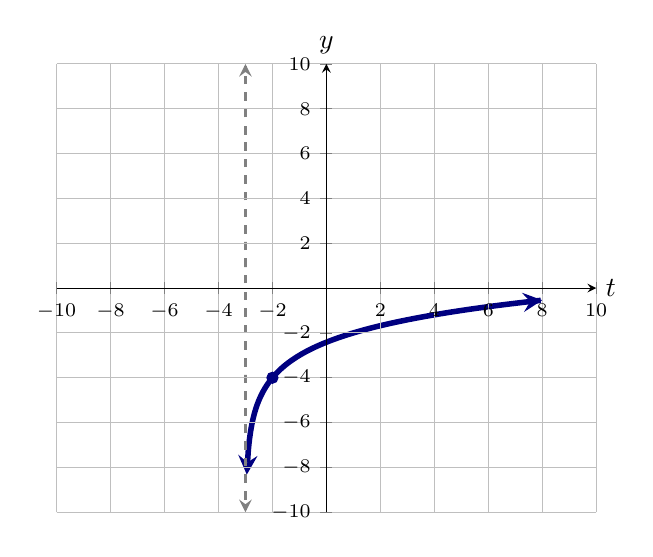
\begin{tikzpicture}
  \begin{axis}[
            domain=-10:10, ymax=10, xmax=10, ymin=-10, xmin=-10,
            axis lines =center, xlabel=$t$, ylabel=$y$, grid = major,
            ytick={-10,-8,-6,-4,-2,2,4,6,8,10},
            xtick={-10,-8,-6,-4,-2,2,4,6,8,10},
            ticklabel style={font=\scriptsize},
            every axis y label/.style={at=(current axis.above origin),anchor=south},
            every axis x label/.style={at=(current axis.right of origin),anchor=west},
            axis on top
          ]
          

			\addplot [line width=2, penColor, smooth,samples=200,domain=(-2.95:8),<->] {ln(x+3)/ln(2)-4};
			%\addplot [line width=2, penColor2, smooth,samples=200,domain=(-8:-0.25),<->] {2^(x+4)-3};


            %\addplot [line width=1, gray, dashed,samples=200,domain=(-10:10),<->] ({x},{-3});
            %\addplot [line width=1, gray, dashed,samples=200,domain=(-10:10),<->] ({x},{x});


			\addplot[color=penColor,fill=penColor,only marks,mark=*] coordinates{(-2,-4)};
			%\addplot[color=penColor2,fill=penColor,only marks,mark=*] coordinates{(-4,-2)};

      \addplot [line width=1, gray, dashed,samples=200,domain=(-10:10),<->] ({-3},{x});






           

  \end{axis}
\end{tikzpicture}
\end{image}




In other words, each function value in a basic logarithmic function occurs exactly once.


If you know that $\log_a(r) = \log_a(t)$, then $r=t$ follows. \\


This is an important rule.





\begin{fact} \textbf{\textcolor{blue!75!black}{Uniqueness}} 


\[     \text{If } \,  \log_a(r) = \log_a(t), \,  \text{ then }  \, r=t    \]


\end{fact}

















\begin{example} Solving Equations


Solve $\log_5(21 + x) = 2$


\begin{explanation}


$\log_5(21 + x) = 2$

$5^{\log_5(21 + x)} = 5^2$

$21 + x = 5^2 = 25$, using the definition of logarithm.

$x = 4$
\end{explanation}
\end{example}










\begin{example} Solving Equations


Solve $\log_2(y) + \log_2(y-4) = \log_2(y+6)$

\begin{explanation}


$\log_2(y) + \log_2(y-4) = \log_2(y+6)$

$\log_2(y(y-4)) = \log_2(y+6)$

$y(y-4) = y+6$    

$y^2 - 4y - y - 6 = 0$

$y^2 - 5y - 6 = 0$

$(y-6) \left( \answer{y+1} \right) = 0$


Either $y-6 = 0$ or $y+1 = 0$

Either $y = 6$ or $y = -1$

However, $y \ne -1$, since $\answer{-1}$ is not in the domain of $\log_2(y)$.

Therefore, just one solution: $6$.

The solution set is $\{ 6 \}$
\end{explanation}
\end{example}






\begin{example} Solving Equations


Solve $7^k = 5$


\begin{explanation}


We are looking for the number that you raise $7$ to, to get $5$.  That number  is $\log_7(5)$.
\end{explanation}
\end{example}















\subsection*{Change of Base}


Logarithms are exponents.  We use them to write expressions in exponential form.



\begin{quote}

Any positive number, $b$, can be written as a power of another positive number, $a$.

\[    b = a^{\log_a(b)}  \]

\end{quote}

For this to be useful, we will need to write multiple expressions with the same base. Therefore, changing the base becomes important.

How do we write $\log_a(b)$ in terms of $\log_c(x)$?




First, $a$ and $b$ can be written in terms of some third base, $c$, using logarithms.


\[    b = c^{\log_c(b)} \,   \text{ and } \,      a = c^{\log_c(a)}      \]



Second, substitute these in for the $a$ and $b$ bases in $b = a^{\log_a(b)}$.



\[   c^{\log_c(b)} = \left(c^{\log_c(a)}\right)^{\log_a(b)}  \]



\[   c^{\log_c(b)} = c^{\log_c(a) \cdot \log_a(b)}  \]



\[   \log_c(b) = \log_c(a) \cdot \log_a(b)  \]


\[   \frac{\log_c(b)}{\log_c(a)} =  \log_a(b)  \]


This is known as the \textbf{Change of Base Formula}.








\begin{template}  Change of Base Formula

\[   \log_a(b)  =  \frac{\log_c(b)}{\log_c(a)}        \, \text{ for } \, a, b, c  > 0        \]


\end{template}











\begin{example}


Write $\log_3(5)$ in terms of logarithms base $7$.


\begin{explanation}


Following the change of base template: $\log_a(b)  =  \frac{\log_c(b)}{\log_c(a)} $ gives



\[   \log_3(5)  =  \frac{\log_7(5)}{\log_7(3)}         \]



\end{explanation}
\end{example}


















$\blacktriangleright$ It occured to people: If we can write any power in terms of any base, and any logarithm in terms of any base, then let's just pick one base to write everything in.


We have such a base: $e$


\section*{e}



\begin{fact} $e$ was defined in a very weird way.

\[   e = \lim_{x \to \infty}  \left(\answer{1 + \frac{1}{x}}\right)^x      \]

\end{fact}




It is weird now.  But as you continue through Calculus, you will see $e$ pop up all over the place.  It seems to have a connection to everything.  So much so that scientists, engineers, and mathematicians have  adopted $e$ as the prefered base for everything.


This means that we encounter $\log_e(x)$ a lot.  And, any time something appears a lot in mathematics, it usually gets a shortcut abbreviation.




\begin{definition}  \textbf{\textcolor{green!50!black}{Natural Logarithm}} 


\[     \ln(x) = \log_e(x) \]


That is a lowerscase ``el'' and a lowercase ``en''.


\end{definition}



\begin{warning}
That is not an uppercase ``eye''.  It is not In.  \\

It is a lowercase ``el'', ln.
\end{warning}




\begin{example}  base e


$\log_7(5) = \frac{\ln(5)}{\ln(7)}$


\end{example}
Everything can be written in terms of base $e$. \\


Calculators usually have a button titled ``ln'' or ``LN''.  When approximating values of logarithms with other bases, we convert them to natural logarithms.  Then we can use the calculator.









\begin{example}  


Approximate $\log_{13}(61)$


\begin{explanation}


Using the LN button on the calculator, we get $\log_{13}(61) = \frac{\ln\left(\answer{61}\right)}{\ln\left(\answer{13}\right)} \approx 1.602711512$
\end{explanation}
\end{example}








\begin{example}  


Rewrite the expression $3 \cdot 5^{2x + 1}$ in the form $e^{f(x)}$.


\begin{explanation}


$3 = e^{\answer{\ln(3)}}$ \\


$5 = e^{\answer{\ln(5)}}$ \\


\[   3 \cdot 5^{2x + 1} = e^{\ln(3)} \cdot (e^{\ln(5)})^{2x + 1}  =  e^{\ln(3)} \cdot e^{\ln(5) \cdot (2x + 1)}  = e^{\ln(3) + \ln(5) \cdot (2x + 1)} \]


\[  e^{\ln(3) + \ln(5) \cdot (2x + 1)} \] 

\end{explanation}
\end{example}














\begin{center}
\textbf{\textcolor{green!50!black}{ooooo-=-=-=-ooOoo-=-=-=-ooooo}} \\

more examples can be found by following this link\\ \link[More Examples of Properties]{https://ximera.osu.edu/csccmathematics/precalculus1/precalculus1/exponentialProperties/examples/exampleList}

\end{center}

\end{document}
